\section{\label{results}Results}
This section presents the results of this study including the systematic literature review and the application of ECV on industry and academic data collected from the primary studies.
Data extracted from primary studies and the results of the quality evaluation are available in \cite{Rinkevics2011a}.

\subsection{State of Practice in Empirical Studies that use CV or Analyze the Results of CV (RQ 1)\label{rq1}}
The study search resulted in 634 unique studies. The search in databases revealed 180 papers, while an additional 454 papers were discovered using snowball sampling.
The study selection resulted in 40 primary studies. Hence, 94\% of the studies were excluded by the selection criteria.
Snowball sampling revealed 15 or 36\% out of all primary studies.
The study selection criteria and the number of papers excluded by each criterion are shown in Tables~\ref{tab:Paper-search-and} and \ref{tab:Paper-Selection-from}.
In total 163 of 634 studies were excluded because full text was not available.

%The review process was facilitated by the reference management software Mendeley.
All results of the study selection are available online and can be obtained by contacting the authors of this paper.
For each study we specify keywords and databases that were used to find the study.
If a study has been excluded, the exclusion criteria are provided.

The number of papers revealed by each search string and database is
presented in Table~\ref{tab:Number-of-papers}. It should be noted
that several papers were found by more than one search string or in
more than one database. Table~\ref{tab:Number-of-papers} shows that
the search string `cumulative voting' was the most frequently used
in research community to denote CV. Therefore, researchers should use 
or reference this term when discussing CV.

To perform snowball sampling we examined the references of primary studies that were found during the database search.
References were used to search for the papers in the Google and Google Scholar search engines.
Studies that were found in the search and passed the study selection criteria were added to the set of primary studies.

After the primary studies were selected, data extraction and quality evaluation was performed by two researchers.
One researcher examined all studies while the second researcher did quality evaluation and data extraction for 10\% of the studies. 
The studies were randomly selected.
Inter-rater agreement were calculated by means of Krippendorff's alpha coefficient.
Agreement for data extraction results was 0.86 and agreement for the quality evaluation was 0.73.
According to \citet{Krippendorff2004a} it is common to require agreement above 0.8 and the lowest acceptable agreement is 0.667. Therefore, we conclude that the agreement calculated for this study is sufficient.
Ratings of the study setting, correctness, research data availability, and number of prioritization items are presented in Figure~\ref{fig:qeResults}.

\begin{figure}
	\center
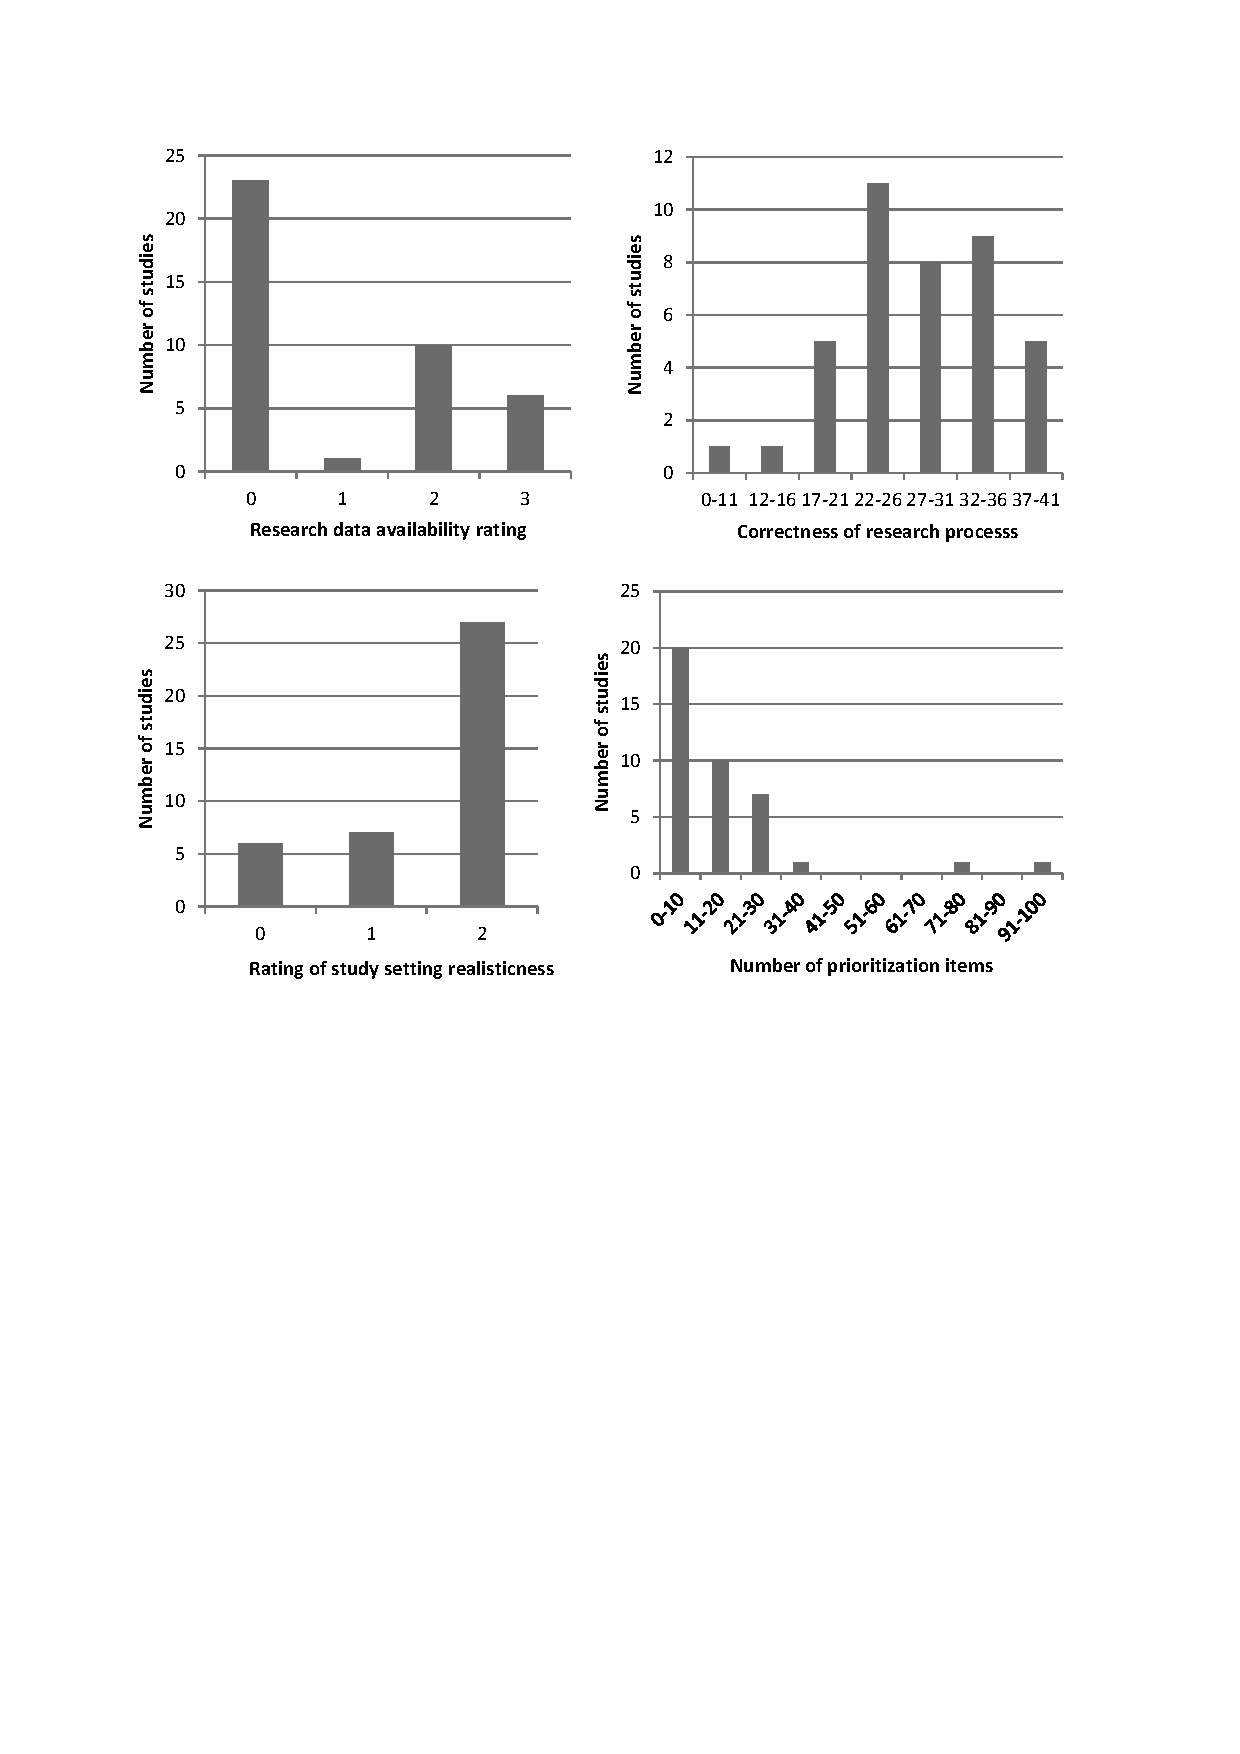
\includegraphics[bb=60bp 360bp 560bp 790bp,clip,scale=0.75]{fig/qeResults}
\caption{\label{fig:qeResults}Study quality ratings}
\end{figure}

\begin{figure}
\center
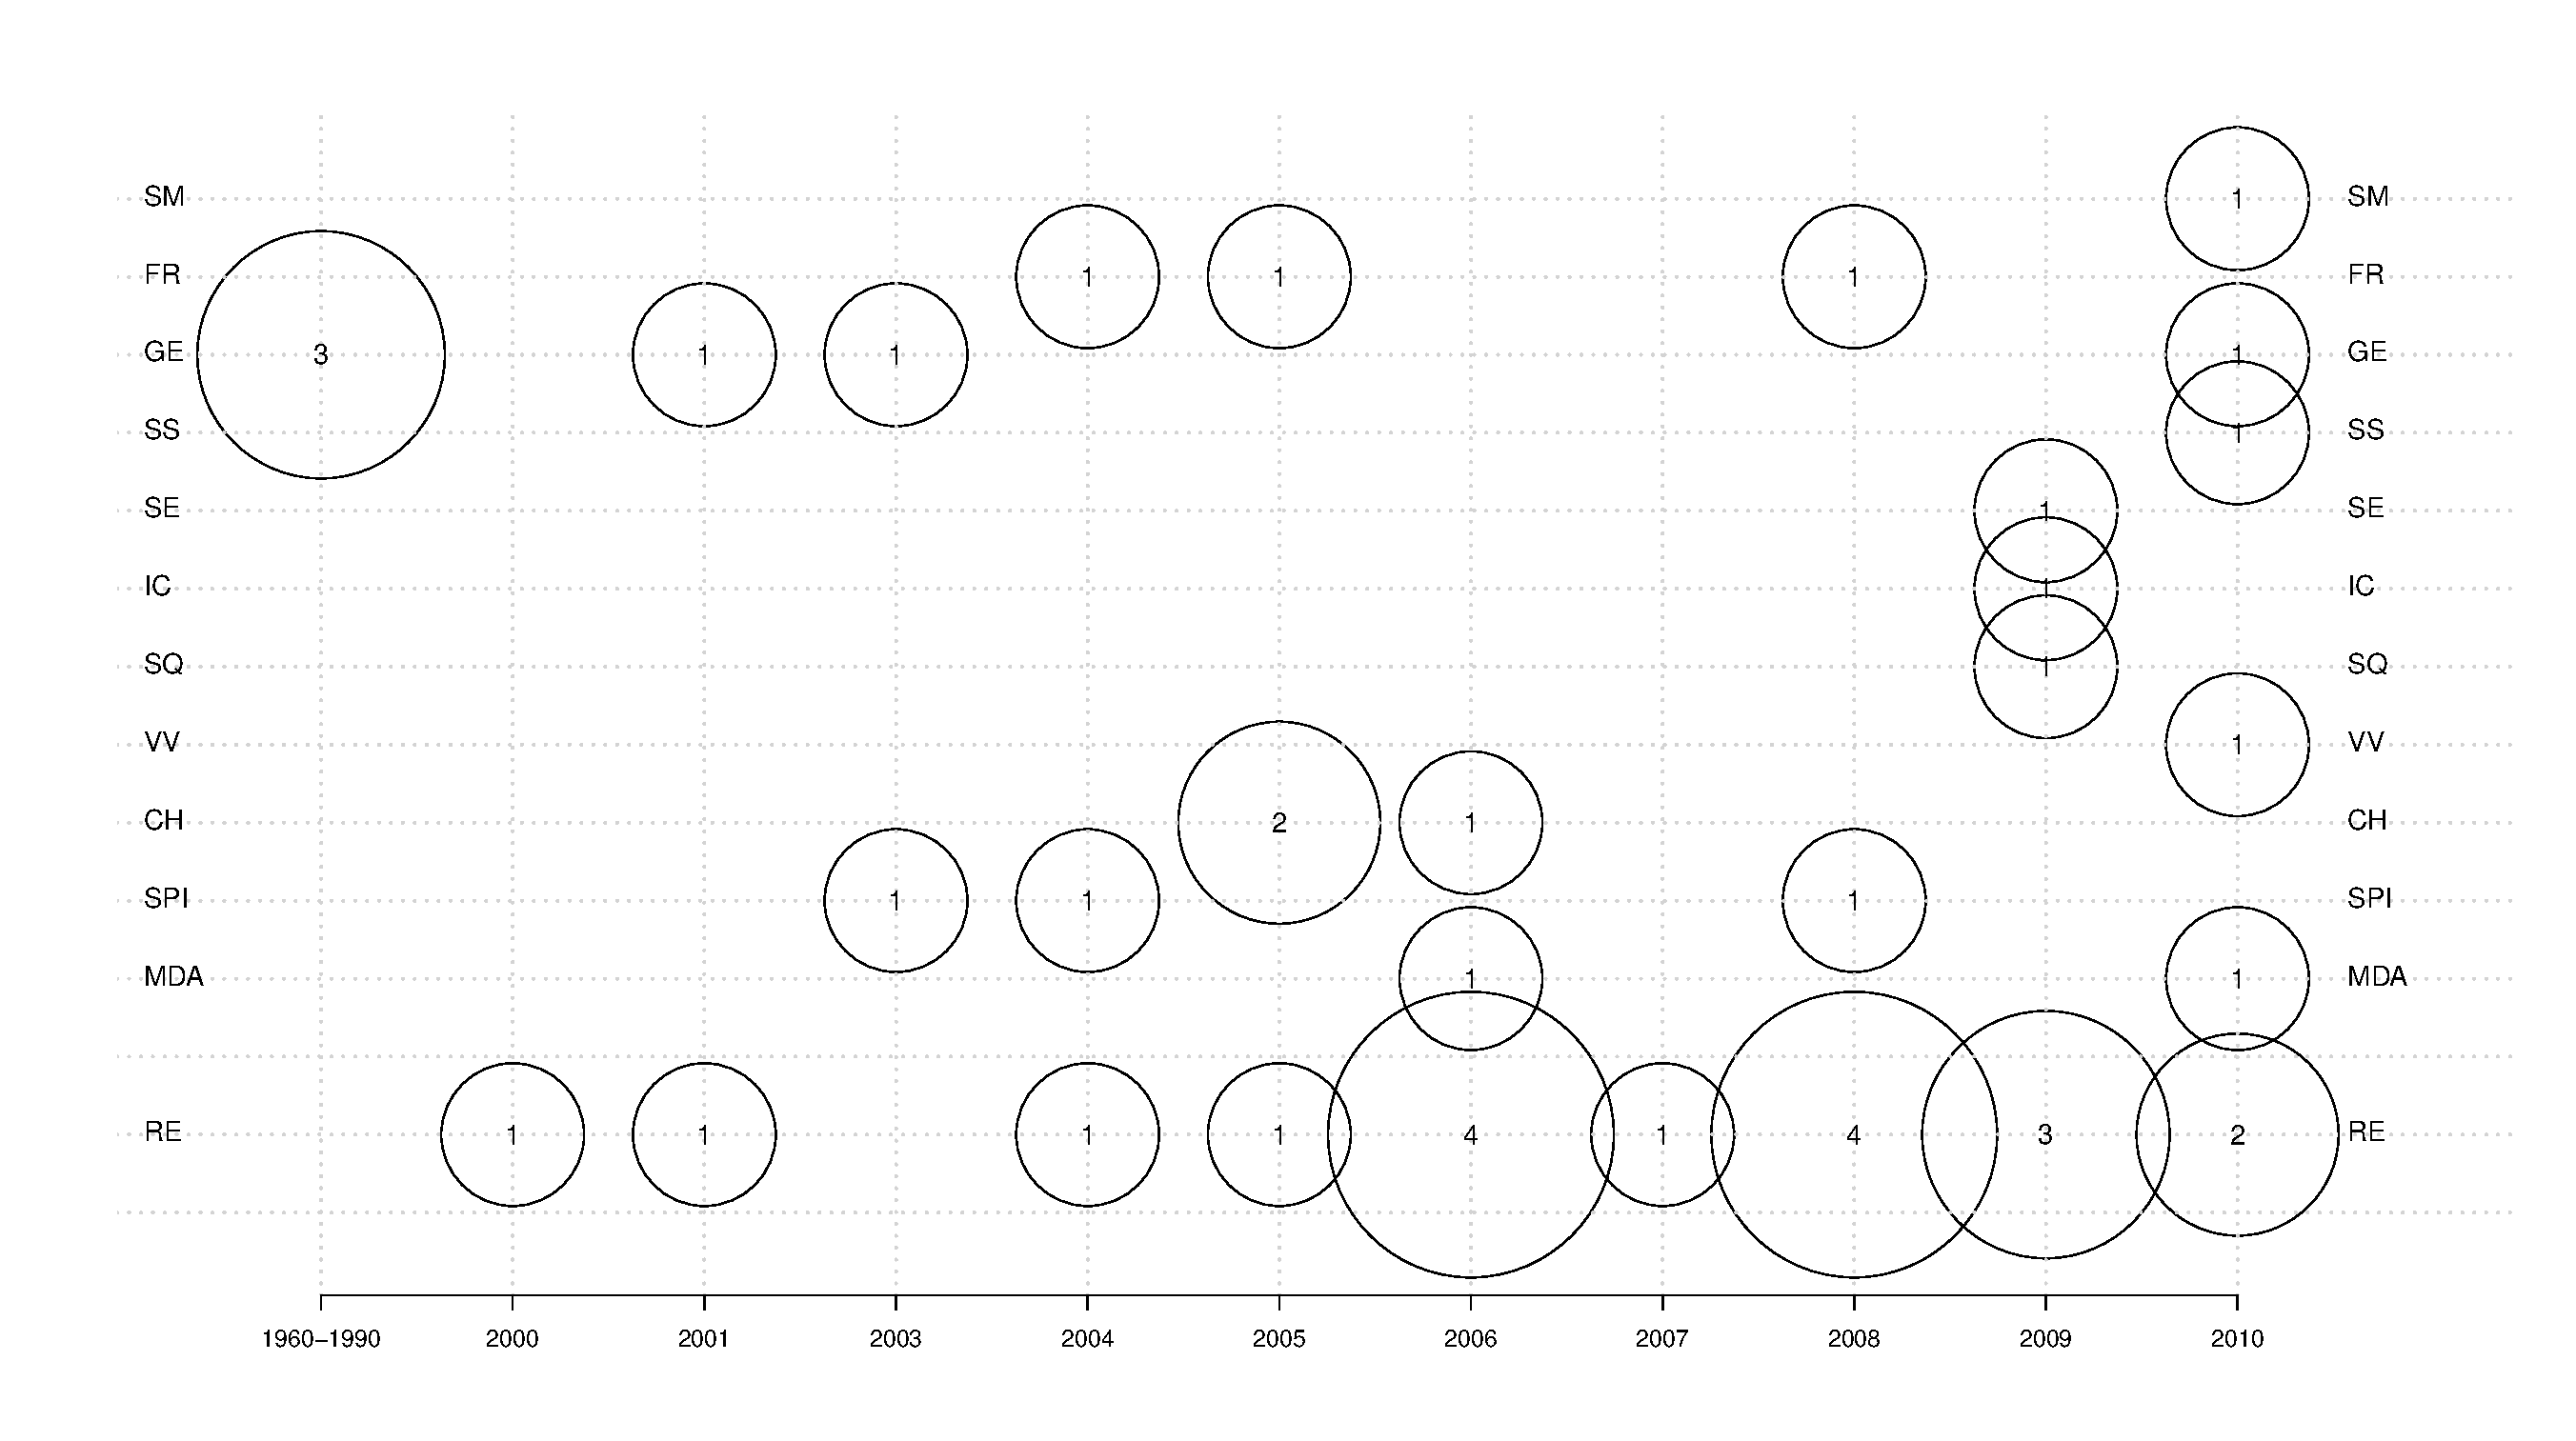
\includegraphics[bb=70bp 40bp 1180bp 670bp,clip,scale=0.28]{fig/bubble}

\begin{tabular}
{l>{\raggedright}b{0.4\columnwidth}l>{\raggedright}b{0.4\columnwidth}l} 
&\tabularnewline
\tiny
MDA - model driven software development  					& \tiny FR - forestry  \tabularnewline
\tiny CH - change impact analysis in software engineering 			& \tiny GE - government elections \tabularnewline
\tiny RE - requirements engineering and software release planning 	& \tiny SS - software security \tabularnewline
\tiny IC - intellectual capital in software company 				& \tiny SQ - software quality \tabularnewline
\tiny SPI - software process improvement 						& \tiny SM - software metrics \tabularnewline
\tiny V\&V - software verification and validation & \tiny SE - software engineering in general\tabularnewline
\end{tabular}
\caption{\label{fig:bubble}Distribution of studies over time.}

\end{figure}

Table~\ref{tab:Top-ranked} shows the studies with the highest quality according to our criteria.
These studies show a high level of rigor in a realistic setting. Moreover, authors of the studies manifest confidence by providing raw data for further use and evaluation.

Figure~\ref{fig:bubble} shows a bubble chart of the distribution of studies over research areas and time.
The figure shows that CV was first applied some time ago in research of government elections.
Nowadays, though, CV has been adopted in a wide range of software engineering areas.
Most frequently in requirements engineering and software release planning.
Eight studies use CV as a research method while the remaining 32 studies report on using CV in industry.

%\begin{flushleft}
%
\begin{center}
\begin{table}

	\scriptsize
\caption{\label{tab:Number-of-papers}Number of papers found in the databases.}

%\raggedright{}
\begin{tabular}{|>{\raggedright}b{0.3\columnwidth}|>{\raggedright}p{0.03\columnwidth}|>{\raggedright}p{0.03\columnwidth}|>{\raggedright}p{0.03\columnwidth}|>{\raggedright}p{0.03\columnwidth}|>{\raggedright}p{0.03\columnwidth}|>{\raggedright}p{0.03\columnwidth}|>{\raggedright}p{0.03\columnwidth}|>{\raggedright}p{0.03\columnwidth}|>{\raggedright}p{0.03\columnwidth}|}
\hline 
 & \multicolumn{7}{l|}{search strings} &  & \tabularnewline
\cline{2-8} 
database & \begin{sideways}
{}``100 point method''%
\end{sideways} & \begin{sideways}
{}``100 dollar method''%
\end{sideways} & \begin{sideways}
{}``100 dollar test''%
\end{sideways} & \begin{sideways}
{}``hundred point method''%
\end{sideways} & \begin{sideways}
{}``hundred dollar method''%
\end{sideways} & \begin{sideways}
{}``hundred dollar test''%
\end{sideways} & \begin{sideways}
{}``cumulative voting''%
\end{sideways} & \begin{sideways}
unique papers found%
\end{sideways} & \begin{sideways}
primary studies selected%
\end{sideways}\tabularnewline
\hline
ACM & 2 & 0 & 0 & 1 & 2 & 3 & 31 & 34 & 7\tabularnewline
\hline 
IEEE & 3 & 2 & 0 & 1 & 2 & 6 & 38 & 46 & 11\tabularnewline
\hline 
Inspec\slash Compendex & 1 & 0 & 0 & 1 & 1 & 1 & 22 & 14 & 7\tabularnewline
\hline 
ISI web of science & 0 & 0 & 0 & 0 & 1 & 1 & 15 & 16 & 6\tabularnewline
\hline 
SCOPUS & 2 & 0 & 0 & 0 & 1 & 2 & 24 & 25 & 9\tabularnewline
\hline 
Springer & 2 & 0 & 2 & 0 & 2 & 2 & 89 & 95 & 6\tabularnewline
\hline 
unique papers found & 6 & 2 & 2 & 1 & 4 & 11 & 165 & 180 & \tabularnewline
\hline 
primary studies selected & 1 & 2 & 1 & 1 & 2 & 4 & 18 &  & 25\tabularnewline
\hline
\end{tabular}%
\end{table}
\end{center}
%\par\end{flushleft}
%
\begin{table}
	\center
	\scriptsize
\caption{\label{tab:Top-ranked}Top ranked studies.}

\begin{tabular}{|>{\raggedright}p{0.24\columnwidth}|>{\centering}p{0.15\columnwidth}|>{\centering}p{0.15\columnwidth}|
>{\centering}p{0.13\columnwidth}|>{\centering}p{0.15\columnwidth}|}
\hline 
 & Correctness of research process & Research data availability & Study setting & Number of prioritization items\tabularnewline
\hline
\citet{Barney2009a} & 36 & 2 & 2 & 17\tabularnewline
\hline
\citet{Berander2009a} & 41 & 2 & 0 & 29\tabularnewline
\hline
\citet{Barney2009} & 40 & 2 & 2 & 5\tabularnewline
\hline
 \citet{Barney2009b} & 31 & 2 & 2 & 27\tabularnewline
\hline
\citet{Barney2008} & 34 & 2 & 2 & 14\tabularnewline
\hline
\citet{Laukkanen2005a} & 22 & 3 & 2 & 30\tabularnewline
\hline
\citet{Hu2006} & 34 & 2 & 1 & 14\tabularnewline
\hline
\citet{Feldt2010} & 24 & 3 & 2 & 8\tabularnewline
\hline
\citet{Regnell2001} & 21 & 3 & 2 & 91\tabularnewline
\hline
\citet{Svahnberg2008} & 34 & 1 & 1 & 7\tabularnewline
\hline
\end{tabular}
\end{table}